\section{Protocol design}
The protocol designed for the system described in this report is based on the examination of networks in Chapter \ref{fig:topologies}, and on the protocols described in Chapter \ref{cha:comprot}.

The network type chosen for the system uses the tree topology, which utilizes a main node, called the root, and multiple branches and leaves. The nodes in the tree does not necessarily connect to the main node, but relays information between the nodes, which is necessary due to the small range of the radio modules used in the solution.

The protocol uses flooding to relay data. When data is requested from the main node, the main node sends a packet requesting sensor readings. The nodes that receive this packet is the first level nodes in the tree. These nodes then read the moisture values from the sensors attached to the nodes, and transmit these back to the main node. 

The first level nodes then request data from the nodes in their vicinity. The nodes receiving this request now has a parent, which is the node that requested data. These nodes are now second-level nodes. The second level nodes read from the sensors, and sends data back to their parents. The parents then relay the data to the main node.

Every time data is request from the main node, the levels are determined again as they might have changed.

\begin{figure}[!h]
	\centering
	\makebox[\textwidth][c]{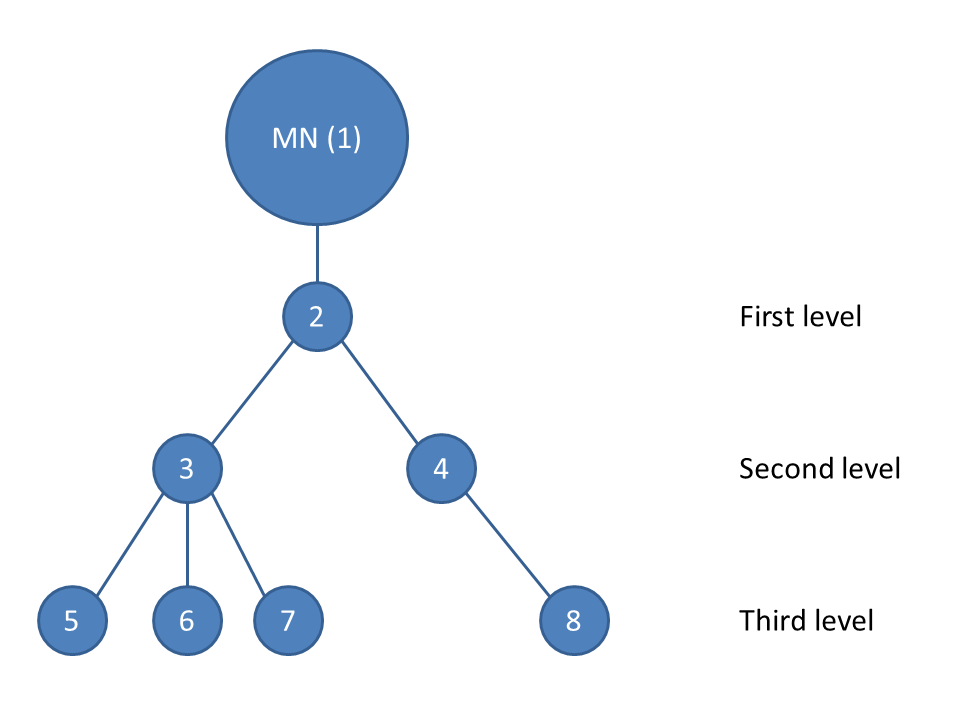
\includegraphics[width=1\textwidth]{chapters/design/figures/prottree1.png}}
	\caption{Example of a tree.}
	\label{fig:prottree1}
\end{figure}

This continues until all reachable nodes have relayed data to the main node.
An illustration showing an example of a tree is seen on Figure \ref{fig:prottree1}.

\subsection*{Adding and removing nodes}
When a new node is added to the network, it needs an identifier in the system. This identifier is provided by the main node, by pairing the device with the main node before adding it onto the golf course. 
This identifier is remembered by the node, and attached to every packet sent by the node.

The identifier is used to determine what node should receive and relay the packets when reading sensor data. On Figure \ref{fig:prottree1}, the nodes 5, 6, and 7, would send packets containing the parent identifier 3. This means that other nodes in the vicinity will ignore these packets, and only node 3 reacts on the packets. Node 3 would then relay the data to node 2, as 2 is its parent, and so on.

Should a node disconnect or be removed from the network, the nodes connected to this node will receive the packets from another node, and from that point on use that as the parent. This is, of course, if there is any nodes in range of the disconnected nodes' subnodes. 

\begin{figure}[!h]
	\centering
	\makebox[\textwidth][c]{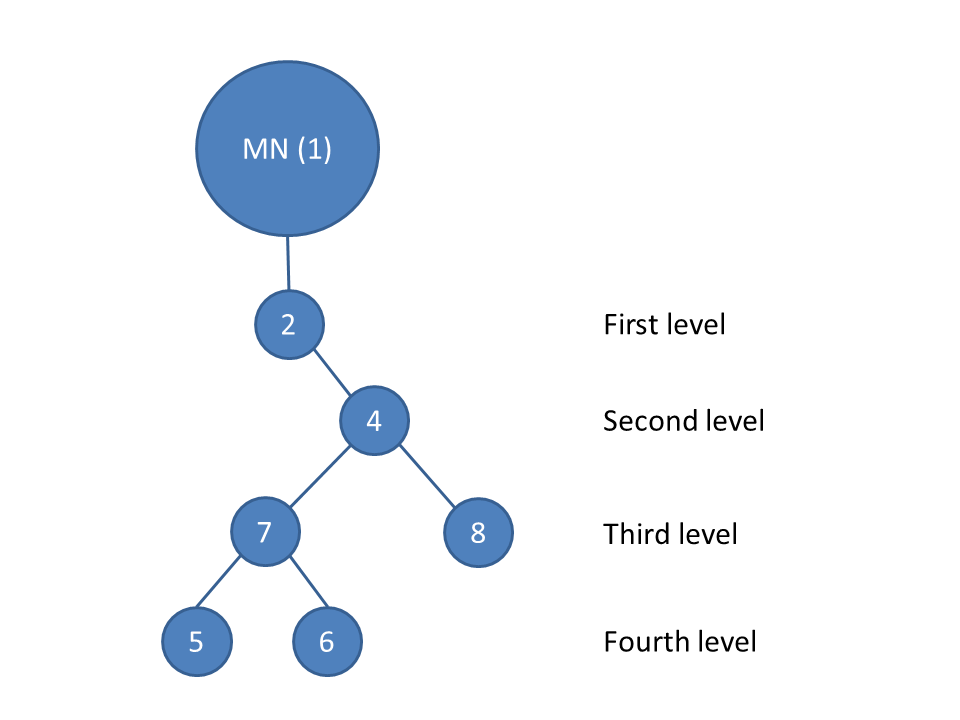
\includegraphics[width=0.8\textwidth]{chapters/design/figures/prottree2.png}}
	\caption{Example of a where node 3 disconnected.}
	\label{fig:prottree2}
\end{figure}

En example of this can be seen on Figure \ref{fig:prottree2}. This figure shows how node 3 disconnected, and now node 7 is attached to node 4 instead. This, of course, assumes that node 7 was in range of node 4.
This means that the next time data is requested, node 7 will be the parent for node 5 and 6, and they will now be a level higher than before.

\subsection*{Interference}
When using a flooding protocol, interference can become a problem, as explained in Chapter \ref{cha:floodingSec}. This occurs even when using controlled flooding, but using a protocol can help reduce problems with interference.

Interferences might cause packets to get mixed up, which makes it impossible to use the data received. Figure \ref{fig:prottree1} shows en example of possible interference. Nodes 5, 6, and 7 could send packets at the same time, causing node 3 to get scrambled data.

To ensure this is not a problem, a checksum is used for verifying packets. This checksum is transmitted with the data and recipient. When a node receives a packet, this checksum is calculated, and compared to the one in the packet. If the checksums match, the packet is accepted and can be relayed to the next node. This will cause the receiving node to send an acknowledgement to the node that sent the packet, which will then stop sending data.
If the checksums does not match, the packet is ignored until a 'clean' packet makes it way to the node.

To ensure that a 'clean' packet will arrive at some point, the nodes will wait a random, but longer, interval between attempting to send data. This means that at some point, the data will get through to the receiver, without interference.
This is possible, as time is not of the essence, and the delay between trying again is small.

\textbf{Wut now?!}
